\normaltrue \difficilefalse \tdifficilefalse
\correctiontrue

%\UPSTIidClasse{11} % 11 sup, 12 spé
%\newcommand{\UPSTIidClasse}{11}

\exer{Écart$\star$ \label{PERF:05:C2:03:509}}
\setcounter{question}{0}\marginnote{\xpComp{PERF}{05}}%\UPSTIcompetence[2]{C2-03}
\index{Compétence C2-03}
\index{Schéma-blocs}
\index{Valeur finale}
\index{Théorème de la valeur finale}
\index{Erreur}
\ifcorrection
\else
\marginnote{\textbf{Pas de corrigé pour cet exercice.}}
\fi


\ifprof 
\else
Soit le schéma-blocs suivant.
\begin{marginfigure}
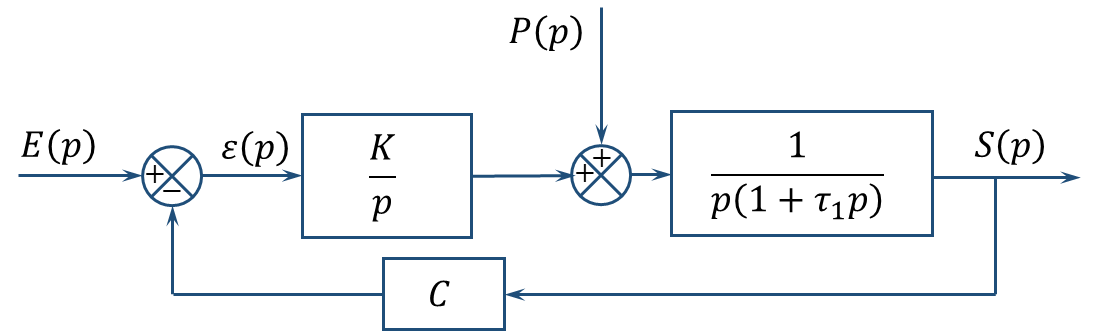
\includegraphics[width=\linewidth]{509_01}
\end{marginfigure}
 \fi
 
\question{Exprimer $\varepsilon(p)$ en fonction de $E(p)$ et $P(p)$.}
\ifprof

On a : 
$\varepsilon(p) = E(p)-C\dfrac{1}{p\left( A+\tau_1 p \right)} \left( \varepsilon(p)\dfrac{K}{p} + P(p)\right)$

$\Leftrightarrow \varepsilon(p) \left(1 +C\dfrac{K}{p^2\left( A+\tau_1 p \right)}\right) = E(p)-C\dfrac{1}{p\left( A+\tau_1 p \right)}  P(p)$

$\Leftrightarrow \varepsilon(p) = E(p)\dfrac{1}{1 +C\dfrac{K}{p^2\left( A+\tau_1 p \right)}}-C\dfrac{1}{p\left( A+\tau_1 p \right)} \dfrac{1}{1 +C\dfrac{K}{p^2\left( A+\tau_1 p \right)}} P(p)$

$\Leftrightarrow \varepsilon(p) = E(p)\dfrac{1}{1 +C\dfrac{K}{p^2\left( A+\tau_1 p \right)}}-\dfrac{C}{p\left( A+\tau_1 p \right) +C\dfrac{K}{p}} P(p)$


\else 
\fi

\question{Évaluer la valeur finale de $\varepsilon(t)$ lorsque $E(p)$ est un échelon d'amplitude $E_0$ et $P(p)$ est un échelon d'amplitude $P_0$.}
\ifprof

On a $\lim\limits_{t\to +\infty} \varepsilon(t) = \lim_{p\to 0} p\varepsilon(p)$.

Dans ces conditons, 
$\varepsilon(p) = E_0\dfrac{1}{p +C\dfrac{K}{p\left( A+\tau_1 p \right)}}-\dfrac{C}{p^2\left( A+\tau_1 p \right) +CK} P_0$.

Au final, $\varepsilon = E_0\dfrac{p}{p +C\dfrac{K}{p\left( A+\tau_1 p \right)}}-\dfrac{Cp}{p^2\left( A+\tau_1 p \right) +CK} P_0$ $=0-0 =0$
\else 
\fi

\question{{Évaluer la valeur finale de $\varepsilon(t)$ lorsque $E(p)$ est un échelon d'amplitude $E_0$ et $P(p)$ est une rampe de pente $P_0$.}
}
\ifprof

Dans ces conditons, 
$\varepsilon(p) = E_0\dfrac{1}{p +C\dfrac{K}{p\left( A+\tau_1 p \right)}}-\dfrac{C}{p^3\left( A+\tau_1 p \right) +CKp} P_0$

et  $\varepsilon = p^2E_0\dfrac{1}{p^2 +C\dfrac{K}{\left( A+\tau_1 p \right)}}-\dfrac{C}{p^2\left( A+\tau_1 p \right) +CK} P_0 = 0 - \dfrac{P_0}{K}=- \dfrac{P_0}{K}$
\else 
\fi

\question{{Évaluer la valeur finale de $\varepsilon(t)$ lorsque $E(p)$ est une rampe de pente $E_0$ et $P(p)$ est un échelon d'amplitude $P_0$.}}
\ifprof

Dans ces conditons, 
$\varepsilon(p) = E_0\dfrac{1}{p^2 +C\dfrac{K}{\left( A+\tau_1 p \right)}}-\dfrac{C}{p^2\left( A+\tau_1 p \right) +CK} P_0$.


On a alors $\varepsilon = pE_0\dfrac{1}{p^2 +C\dfrac{K}{\left( A+\tau_1 p \right)}}-\dfrac{C}{p^2\left( A+\tau_1 p \right) +CK} P_0p = 0$


\else 
\fi

\question{{Évaluer la valeur finale de $\varepsilon(t)$ lorsque $E(p)$ est une rampe de pente $E_0$ et $P(p)$est une rampe de pente  $P_0$.}}
\ifprof

Dans ces conditons, 
$\varepsilon(p) = E_0\dfrac{1}{p^2 +C\dfrac{K}{\left( A+\tau_1 p \right)}}-\dfrac{C}{p^3\left( A+\tau_1 p \right) +CKp} P_0$. 
On a alors
$\varepsilon = E_0 p \dfrac{1}{p^2 +C\dfrac{K}{\left( A+\tau_1 p \right)}}-\dfrac{C}{p^2\left( A+\tau_1 p \right) +CK} p P_0 = -\dfrac{P_0}{K} $.

\else 
\fi




%\question{Réaliser le schéma-blocs.}
%\ifprof
%\begin{figure}[H]
%\centering
%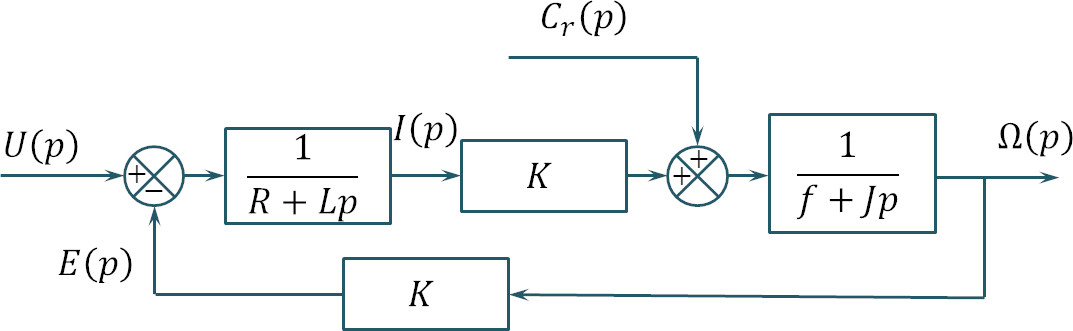
\includegraphics[width=\linewidth]{51_01_c}
%%\caption{Évolution du couple utile en fonction de la vitesse de rotation pour des
%%fréquences de commande de \SI{90}{Hz} à \SI{110}{Hz}. \label{fig_50_04}}
%\end{figure}
%\else
%\fi


 

\ifprof
\else

\marginnote{Corrigé voir \ref{PERF:05:C2:03:509}.}

\fi